\subsection{Template-Method}

\subsubsection*{Problembeschreibung}

Ein Algorithmus besteht aus mehreren Schritten, die jeweils eine bestimmte Aufgabe erfüllen. Diese Schritte können je nach Situation oder Anforderung unterschiedlich implementiert werden, ohne den Algorithmus zu verändern. Der Algorithmus legt jedoch die Abfolge der Schritte fest und ruft sie in einer vorgegebenen Reihenfolge auf. \cite{gamma_design_1995}

\subsubsection*{Lösung}

Jede Klasse, welche einen Algorithmus der selben Struktur implementiert, erbt von einer abstrakten Klassen (\code{AbstractClass}), welche die \code{templateMethod} implementiert. Das wird in Abbildung \ref{fig:template-method-class} gezeigt. Diese gibt das Grundgerüst des Algorithmus vor und ruft darin die einzelnen Teilschritte auf. Diese sind jeweils in eigenen Methoden implementiert. Die Subklassen (\code{ConcreteClass}) definieren diese Methoden zum Teil neu, wenn eine Veränderung des Verhaltens dieses Teilschrittes notwendig ist.

\begin{figure}[H]
	\centering
	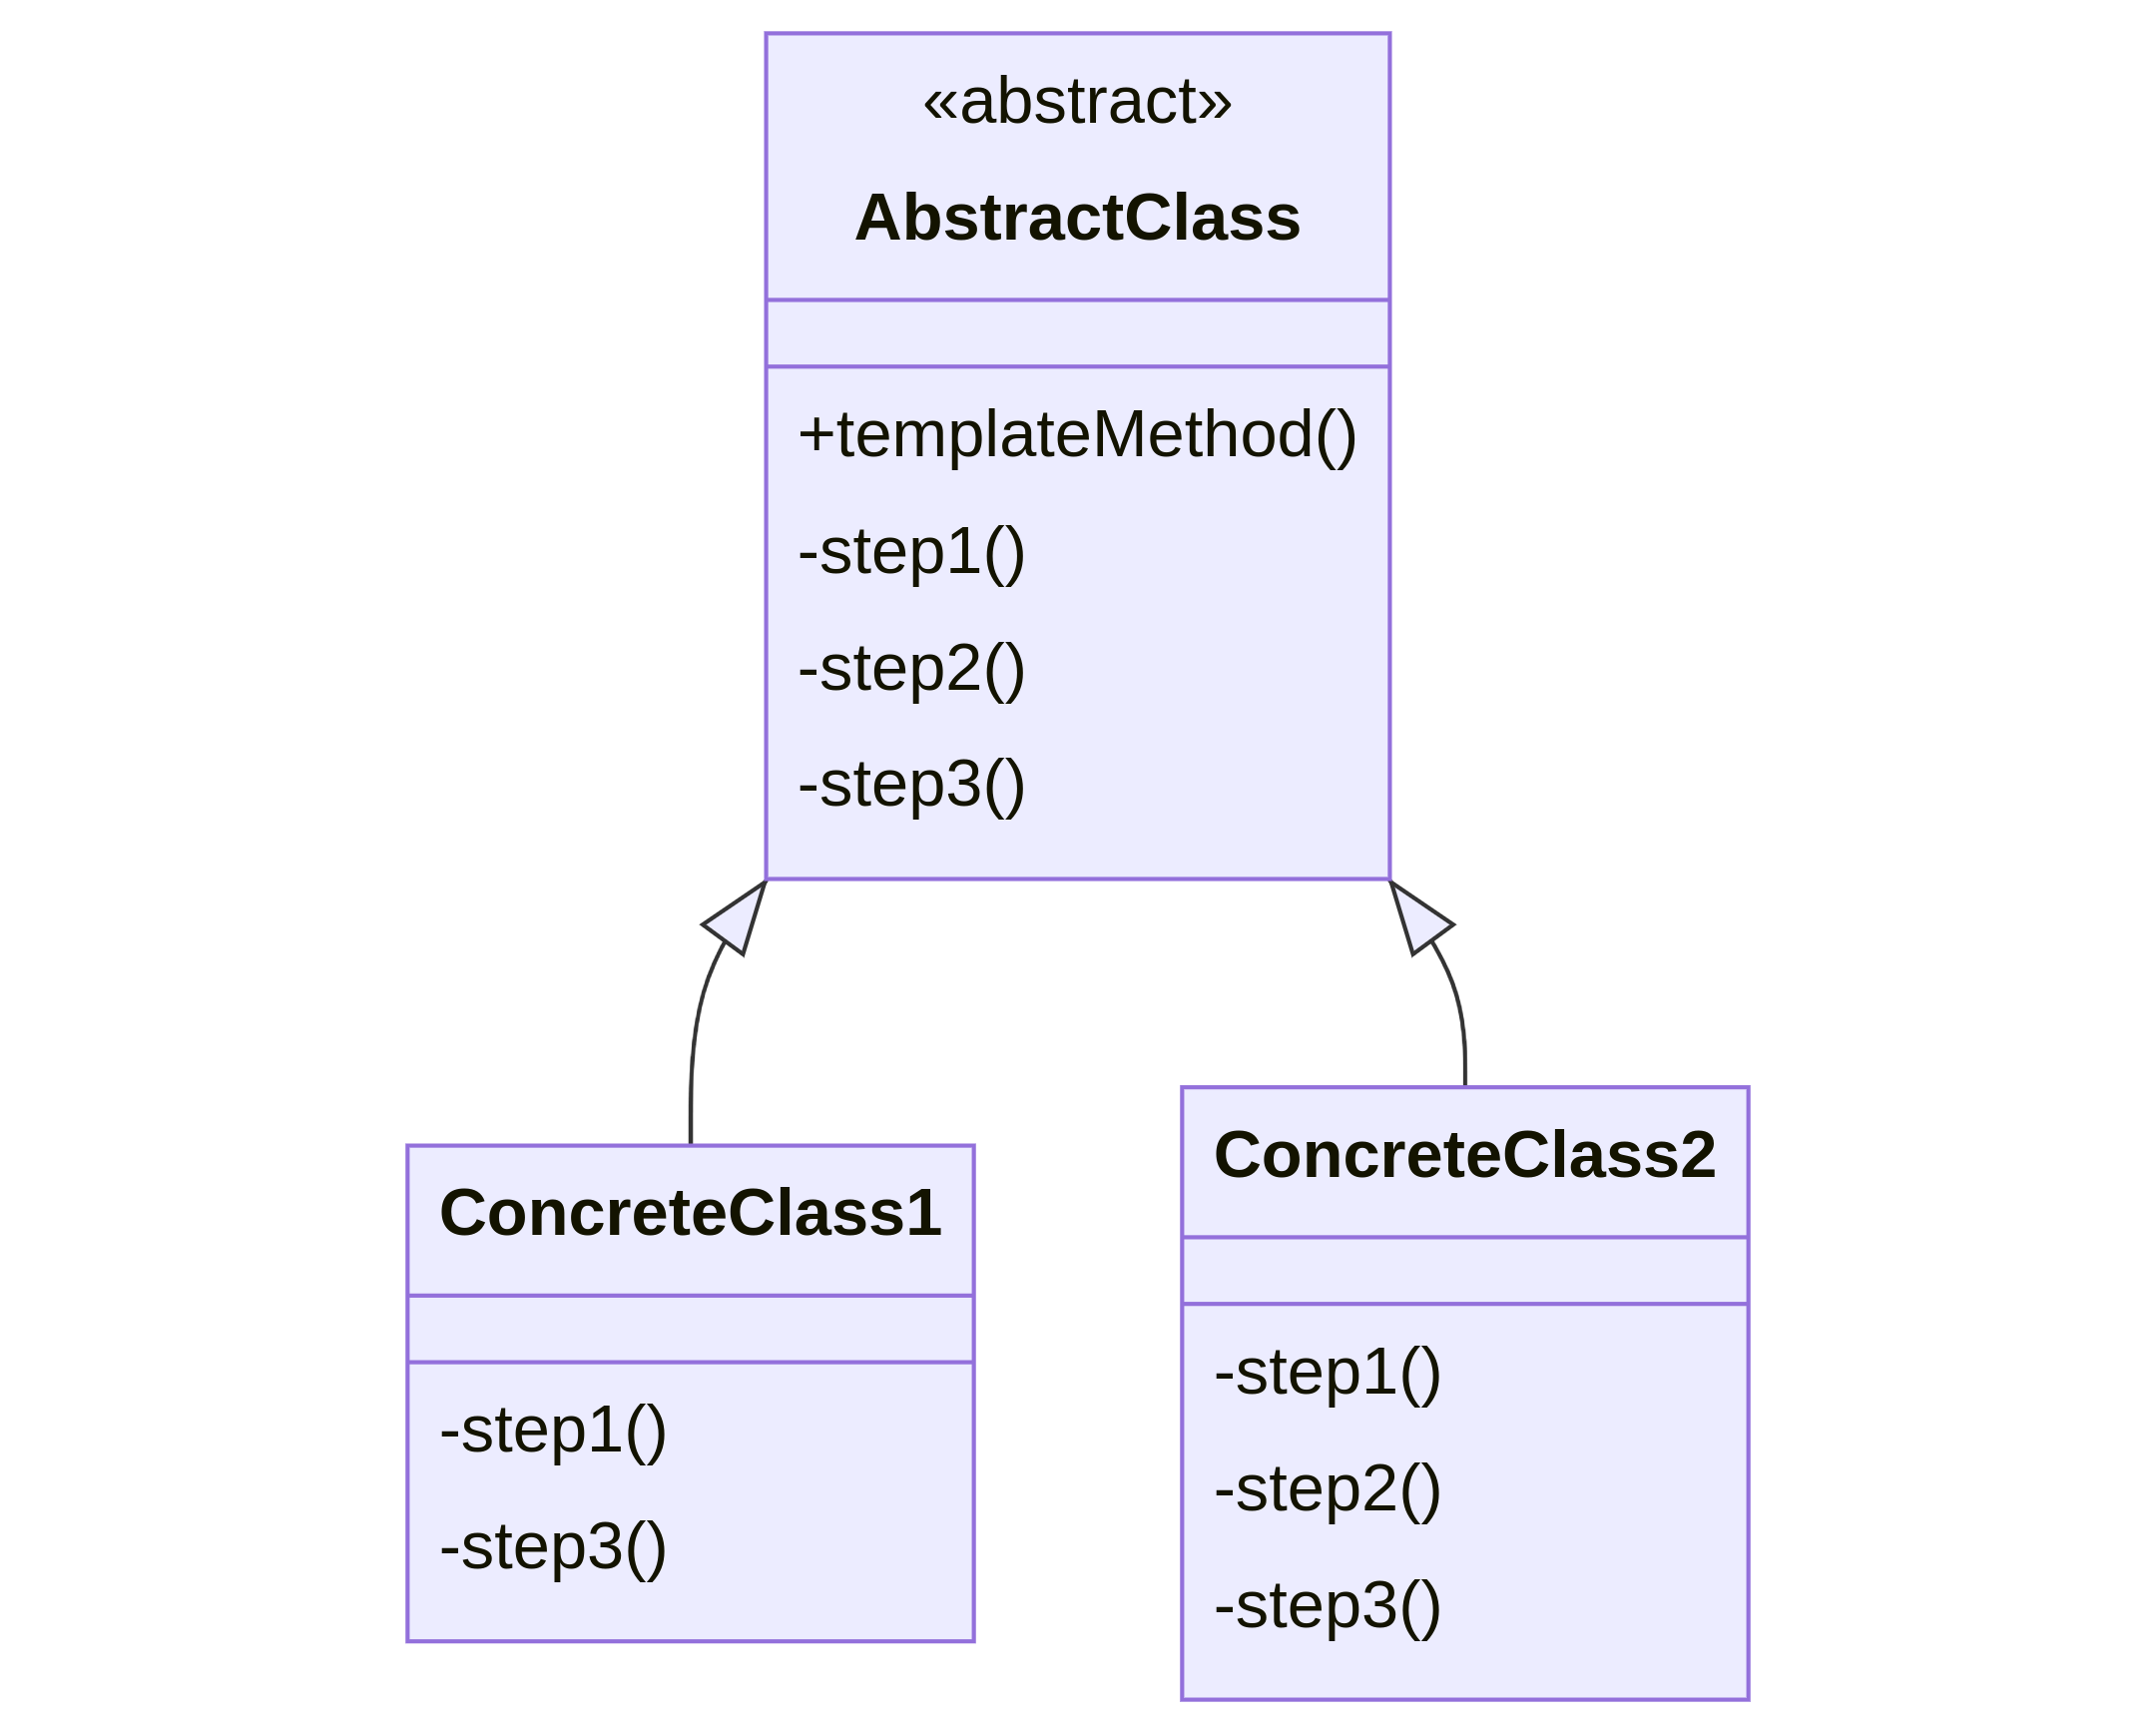
\includegraphics[width=0.75\linewidth]{images/patterns/template-method-class.png}
	\caption{Klassendiagramm der Template-Method \cite{skobeleva_template_2023}}
	\label{fig:template-method-class}
\end{figure}

Quelltext\ref{code:template-method-code} zeigt exemplarisch, wie eine solche \emph{Template-Method} aussehen kann. Die Reihenfolge und Interaktion der drei Einzelschritte \code{step1}, \code{step2} und \code{step3} sind festgelegt. Deren konkretes Verhalten kann jedoch in den Subklassen von \code{AbstractClass} überschrieben werden.

\lstset{language=python}
\begin{lstlisting}[caption={Exemplarische Implementierung einer Template-Method}, label=code:template-method-code]
class AbstractClass:
	def templateMethod(self):
    	if self.step1():
        	self.step2()
    	self.step3()
\end{lstlisting}


\subsubsection*{Konsequenzen}

Template-Methods sind ein Mechanismus, welcher die Wiederverwendung von Code ermöglicht und kann somit der Codeduplikation entgegen wirken. Anstatt Abwandlungen von Algorithmen von Grund auf neu zu implementieren, ist es möglich, sie aus bestehenden Komponenten zusammenzusetzen und je nach Bedarf neuen Code hinzuzufügen. Das Muster der Template-Method weist eine umgekehrte Kontrollstruktur auf. Anstatt dass eine Klasse Methoden ihrer Superklasse aufruft, delegiert die Template-Method die Verantwortlichkeit für die einzelnen Teile des Algorithmus an sie Subklassen.

Bei der Verwendung der Template-Method ist jedoch zu beachten, wie die einzelnen Methoden zu verwenden sind. Diese lassen sich grob in zwei Arten einteilen, die \emph{Hook}\footnote{Schnittstelle zur Integration fremden Codes in ein bestehendes System}-Methoden und die abstrakten Methoden. Während die Hook-Methoden eine Standard-Implementierung in der abstrakten Basisklasse bereitstellen, ist dies bei den abstrakten Methoden nicht der Fall. Entsprechend müssen die abstrakten Methoden zwingend von einer konkreten Subklasse implementiert werden. Bei den Hook-Methoden ist das optional.

Die Template-Method synergiert mit dem Strategy-Pattern. Einzelne Schritte eines Algorithmus können in einer Strategie-Klasse implementiert sein. \cite{gamma_design_1995}